\begin{center}
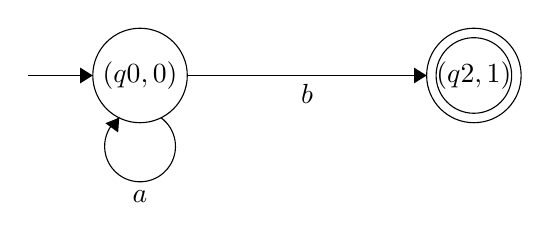
\begin{tikzpicture}[scale=0.2]
\tikzstyle{every node}+=[inner sep=0pt]
\draw [black] (24.1,-24.2) circle (3);
\draw (24.1,-24.2) node {$(q0,0)$};
\draw [black] (45.3,-24.2) circle (3);
\draw (45.3,-24.2) node {$(q2,1)$};
\draw [black] (45.3,-24.2) circle (2.4);
\draw [black] (27.1,-24.2) -- (42.3,-24.2);
\fill [black] (42.3,-24.2) -- (41.5,-23.7) -- (41.5,-24.7);
\draw (34.7,-24.7) node [below] {$b$};
\draw [black] (17,-24.2) -- (21.1,-24.2);
\fill [black] (21.1,-24.2) -- (20.3,-23.7) -- (20.3,-24.7);
\draw [black] (25.423,-26.88) arc (54:-234:2.25);
\draw (24.1,-31.45) node [below] {$a$};
\fill [black] (22.78,-26.88) -- (21.9,-27.23) -- (22.71,-27.82);
\end{tikzpicture}
\end{center}